% Chapter 2 - Background

\glsresetall % reset the glossary to expand acronyms again
\chapter[Literature Review]{Literature Review}\label{ch:LitReview}
\index{Literature Review}

% Literature Review
%\section{Literature Review}

\section{Introduction}

%\begin{itemize}
%    \item \sout{Purpose/scope of lit review. }
%    \item \sout{Areas of lit reviewed. }
%    \item \sout{How the lit review will impact the design.} 
%    \item Boundaries of lit review.
%\end{itemize}
The purpose of this literature review is to survey and investigate relevant literature to aid the design of a smart sunbird feeder. The literature reviewed will inform subsequent design choices and methods. Literature concerning ecological and avian monitoring will support the motivation for research in this area, while identifying sunbird behaviours and characteristics of nectar feeders that may present difficulties or limitations. Existing automated bird-monitoring solutions will be analysed to determine how aspects of similar research can best be applied. Several key enabling technologies will then be investigated, together with their respective advantages and disadvantages. Finally, the literature review will identify important trade-offs in similar projects and address the research gap this project aims to fill. The findings will support informed design and implementation decisions based on the accomplishments and limitations reported in the literature.

\section{Bird monitoring and nectarivorous ecology:}

%\begin{itemize}
%    \item \sout{Importance of monitoring bird activity.}
%    \item \sout{Normal monitoring methods and their limitations.}
%    \item \sout{Benefits of non-invasive monitoring.} 
%    \item \sout{A bit of relevant sunbird behaviour.} 
%    \item \sout{Unique aspects of nectar feeders.} 
%    \item \sout{Ecology/hygiene issues around supplemental feeding.}
%\end{itemize}

Firstly, it is important to establish the relevance of ecological monitoring as motivation for research in this field, which this section aims to accomplish.
\par\vspace{6pt}
Bird activity is a vital metric for determining ecosystem biodiversity and functioning. Nations have adopted methods of observing this activity to support sustainable development strategies and gauge environmental and ecosystem health \cite{GregoryVanStrien2010}. Conventional avian ecological monitoring includes approaches such as human point counts, passive sound recording and camera traps. These methods have proven practically identical in effectiveness when implemented correctly, while remote observation is preferred for remote deployment or rare species monitoring \cite{DarrasEtAl2018}. Sound recording and similar autonomous methods reduce the time required for human monitoring, provide permanent data capture and eliminate human observer bias. These methods also have drawbacks, including equipment and storage costs and the risk of data loss if they fail \cite{ShonfieldBayne2017}. Despite these shortcomings, remote monitoring systems, particularly camera traps, are widely used for wildlife monitoring. Depending on the model, set-up and application, camera traps are viable for a diverse range of scenarios \cite{TrollietEtAl2014}. \textbf{The advantages, limitations and project suitability of these monitoring methods are summarised in} Table~\ref{tab:birdmonitoringmethods}.

\begin{table}[htbp]
    \centering
    \caption{Comparison of common methods used for monitoring bird activity.}
    \label{tab:birdmonitoringmethods}
    
    \small
    \renewcommand{\arraystretch}{1.25}
    
    \begin{tabularx}{\textwidth}{
        >{\raggedright\arraybackslash}p{0.18\textwidth}
        >{\raggedright\arraybackslash}X
        >{\raggedright\arraybackslash}X
        >{\raggedright\arraybackslash}p{0.20\textwidth}
    }
        \toprule
        \textbf{Method}
        & \textbf{Principal advantages}
        & \textbf{Principal limitations}
        & \textbf{Suitability for this project} \\
        \midrule
        
        Human point counts
        & Can identify birds using both visual and acoustic observations; requires relatively little equipment; experienced observers can interpret behaviour and surrounding conditions immediately.
        & Requires trained observers and considerable field time; observations are restricted to scheduled survey periods; susceptible to observer bias; generally provides no permanent visual record.
        & Low. Useful for manually validating system observations, but unsuitable as the primary method for continuous autonomous monitoring. \\
        
        \addlinespace
        
        Passive acoustic monitoring
        & Enables long-duration unattended recording; provides a permanent record; can detect birds that are hidden from view; reduces the need for an observer to remain in the field.
        & Produces large volumes of audio data; performance is affected by background noise and overlapping calls; silent birds cannot be detected; reliable species identification may require specialist analysis or automated classifiers.
        & Moderate. Valuable for monitoring vocal activity, but it cannot provide the visual information required by the proposed image-based classification system. \\
        
        \addlinespace
        
        Camera-trap monitoring
        & Provides permanent visual records; enables verification of species, visit duration and aspects of behaviour; can operate autonomously; supports automated image or video analysis.
        & Detection depends on camera placement and trigger performance; false and missed activations may occur; image quality is affected by lighting, motion and occlusion; video requires substantial storage and energy.
        & High. The predictable feeding location allows the camera field of view and trigger region to be constrained, making this the most appropriate primary monitoring method. \\
        
        \bottomrule
    \end{tabularx}
    
    \vspace{0.5em}
    
    \begin{minipage}{0.96\textwidth}
        \footnotesize
        \textit{Sources:} Comparison informed by Darras et al. 
        \cite{DarrasEtAl2018}, Shonfield and Bayne 
        \cite{ShonfieldBayne2017}, and Trolliet et al. 
        \cite{TrollietEtAl2014}.
    \end{minipage}
\end{table}

\par\vspace{6pt}
In Cape Town, sunbirds have been shown to play a particularly important ecological role, with the four local nectar-feeding species contributing significantly to the maintenance of the region's many bird-pollinated plant species \cite{GeertsEtAl2020}. This role is accompanied by behavioural traits that affect how they should be monitored. Although sunbirds can hover while feeding, they frequently perch near nectar sources when an appropriate platform is available. Providing a perch therefore makes camera-based monitoring more practical \cite{SejfovaEtAl2021}. Sunbirds also associate food-source quality with colour, making feeder appearance more important than for seed-feeding species \cite{WhitfieldEtAl2014}. Many nectar feeders therefore use red feeding ports because red is common among flowers, highly visible in natural settings and less detectable to bees, reducing competition at the food source \cite{ChenEtAl2020}. Sunbird feeding routines also adapt to the location and quality of available food sources. Feeder activity should therefore not be assumed to represent overall sunbird activity in the surrounding area \cite{DuPlessisEtAl2021}. While some studies suggest supplemental feeding may concentrate sunbird activity and affect surrounding pollination networks, others report negligible effects on activity at natural food sources \cite{DuPlessisEtAl2021, MantintsililiEtAl2025}.
\par\vspace{6pt}
Sunbird feeders differ significantly from ordinary seed feeders because these birds are nectarivorous. Their diet requires feeders to contain liquid rather than solid food and, due to their long bills and "tube-like" tongues, they prefer narrow feeding ports over the trays commonly used in seed feeders \cite{CubanEtAl2026}. The nectar solution consists of water supplemented with sugar, particularly sucrose. Studies of sunbird feeder preferences found sucrose-rich solutions to be more popular than hexose-rich alternatives \cite{FlemingEtAl2004}. However, storing nectar in feeders can promote microbial transmission and fermentation, resulting in ethanol production. An analysis of hummingbird feeders found non-pathogenic bacteria and fungi that differed significantly from those found in flowers \cite{LeeEtAl2019}. Additionally, an ethanol concentration of only 2\% was found to significantly reduce sunbird visitation \cite{ChoiEtAl2023}. For these reasons, feeder nectar should be replaced regularly.

\section{Analysis of existing smart bird feeders}

%Focus on 
%\begin{itemize}
%    \item Intended purpose
%    \item Monitoring capabilities
%    \item Feeder type
%    \item Image or video capture
%    \item Species identification
%    \item Embedded operation
%    \item Connectivity and data access
%    \item Power supply
%    \item Outdoor deployment and reliability
%\end{itemize}

This section of the literature review will be dedicated to investigating the efforts of other individuals in similar fields of research and acknowledging the benefits and drawbacks for each of their respective approaches to conducting their research. 
\par\vspace{6pt}

\subsection{Research and experimental smart-feeder systems}
Rapid advances in Machine Learning (ML) and the increasing availability and affordability of microcomputers such as the Raspberry Pi (RPi) have enabled the development of smart bird feeders by both companies and academics. Researchers have demonstrated the feasibility of using an RPi as the computational core of a smart seed feeder, reliably capturing data from visiting birds using video, microphone and strain gauge recordings \cite{NiersEtAl2022}. The system also performed local species inference using an embedded ML algorithm and uploaded data to an independently hosted website for user access and download. However, this approach requires an internet connection for data access, limiting deployment in remote areas. The system also depends on an external power supply, further restricting remote deployment \cite{NiersEtAl2022}.
\par\vspace{6pt}
Another approach to smart bird feeders is to decentralise the computational load by relying on a remote server. By moving computation away from the physical feeder, researchers were able to monitor an unmodified, commercially available seed feeder using a standard internet-enabled camera trap. The Artificial Intelligence (AI) used for identification was also trained only on bird species relevant to the area, substantially reducing computational demand compared to recognising all bird species. Like the previously reviewed feeder, however, the system requires both an internet connection and an external power supply. Although narrowing the training database reduced computational demand, field accuracy fell from 99.5\% to 88\%, emphasising the importance of representative training data \cite{Mansouri2025}.
\par\vspace{6pt}
When shifting focus from seed-feeding to nectar-feeding birds, monitoring approaches often rely on radio-frequency identification (RFID) rather than computer vision and ML. Although RFID enables highly reliable identification, implementation is invasive because tags must be physically attached to the birds. One smart seed feeder using RFID relied on an RPi \cite{Youngblood2019}, while another used a simpler Arduino microcontroller. Because RFID does not require an ML component, the computing power required to operate the system can be significantly reduced \cite{IbarraEtAl2015}.
\par\vspace{6pt}
\subsection{Commercial smart nectar feeders}
Smart bird feeders are not exclusively academic projects, with several commercially available versions now on the market. The Birdbuddy Smart Hummingbird Feeder is one relevant example \cite{BirdBuddyHummingbirdFeeder}. One notable design feature is its colour choice: the feeding port area is made from translucent red plastic, aligning with earlier literature showing that nectar-feeding birds associate food sources with colour. Red is also the most common colour used by feeder manufacturers, further supporting this literature. Another commercial example is the Birdfy Hum Feeder, which has a very similar design \cite{BirdfyHumFeeder}. Both products depend on proprietary software, cloud-based storage, a mobile application and consistent internet access. The principal characteristics, advantages and limitations of the academic and commercial smart bird feeders reviewed are summarised in Table~\ref{tab:existing-smart-feeders}.

\begin{sidewaystable}[p]
\centering
\caption{Comparison of selected academic and commercial smart bird-feeder systems.}
\label{tab:existing-smart-feeders}

```
\small
\setlength{\tabcolsep}{4pt}
\renewcommand{\arraystretch}{1.15}

\begin{tabularx}{\textheight}{
    >{\raggedright\arraybackslash}p{0.13\textheight}
    >{\raggedright\arraybackslash}p{0.09\textheight}
    >{\raggedright\arraybackslash}X
    >{\raggedright\arraybackslash}X
    >{\raggedright\arraybackslash}p{0.11\textheight}
    >{\raggedright\arraybackslash}X
}
    \toprule
    \textbf{System}
    & \textbf{Feeder}
    & \textbf{Monitoring}
    & \textbf{Processing and storage}
    & \textbf{Power}
    & \textbf{Key limitation or lesson} \\
    \midrule

    Niers et al. \cite{NiersEtAl2022}
    & Seed
    & Video, audio and strain-gauge measurements.
    & RPi performs local species classification and uploads results to a hosted website.
    & External supply.
    & Demonstrates non-invasive multimodal monitoring, but requires network access and external power. \\

    Mansouri \cite{Mansouri2025}
    & Seed
    & Motion-triggered IP camera recording short videos.
    & Videos are transferred to a local server for bird detection and classification of 40 local species.
    & Off-grid supply not specified.
    & Localised training reduces computational demand, but field accuracy fell from 99.5\% to 88\%. \\

    Youngblood \cite{Youngblood2019}
    & Seed
    & Perch-mounted RFID detects tagged birds.
    & RPi Zero W stores tag identifiers and timestamps.
    & Portable battery.
    & Enables reliable individual identification, but requires invasive tagging and cannot identify untagged birds. \\

    Ibarra et al. \cite{IbarraEtAl2015}
    & Nectar
    & RFID detection with servo-controlled feeding port.
    & Microcontroller controls access and stores tag identifiers and timestamps on an SD card.
    & Two 9~V batteries.
    & Enables low-power local operation, but requires invasive tagging and provides no visual identification. \\

    Birdbuddy Smart Hummingbird Feeder
    \cite{BirdBuddyHummingbirdFeeder}
    & Nectar
    & Automatic photo and video capture.
    & Proprietary identification software with recordings accessed through a mobile application.
    & Rechargeable battery; optional solar.
    & Polished consumer system, but depends on proprietary software and network connectivity. \\

    Birdfy Hum Feeder
    \cite{BirdfyHumFeeder}
    & Nectar
    & Motion-triggered 1080p video and automated identification.
    & Recordings and results are accessed through a proprietary application.
    & Rechargeable battery; optional solar.
    & Demonstrates solar-supported monitoring, but depends on proprietary software and connectivity. \\

    \bottomrule
\end{tabularx}
```

\end{sidewaystable}

\par\vspace{6pt}
\subsection{Comparative findings and design implications}
An investigation of existing smart bird feeders, developed for either research or commercial purposes, reveals several recurring design choices and limitations. Although most available literature concerns seed feeders, smart nectar feeders have also been developed. Most systems rely on a microcomputer, typically an RPi, rather than a microcontroller to implement ML-based, non-invasive species identification. Another common design choice is to offload data storage and user interaction to an external or cloud-based server rather than hosting locally. This reduces local computational overhead but requires an internet connection. Nearly all inspected systems also rely on a constant external power source, severely limiting deployment in remote areas.

\clearpage

\section{Technology behind autonomous bird monitoring systems}

This section will refine upon the broader topic of existing smart feeders discussed in the previous section and will focus on several of the technologies that comprise the functional pipeline of such feeders. The design choices behind the technology at each stage of this pipeline will be investigated in order to better inform the design of this project. The principal stages of a generic autonomous bird-monitoring pipeline are illustrated in Figure~\ref{fig:generic-monitoring-pipeline}.

\begin{figure}[H]
    \centering
    \begin{tikzpicture}[
        scale=0.76,
        transform shape,
        font=\small,
        >=Latex,
        line/.style={draw=black!70,line width=0.9pt,-{Latex[length=2.5mm]}},
        optional/.style={line,dashed},
        process/.style={
            rectangle,
            rounded corners=2mm,
            draw=black!65,
            line width=0.8pt,
            align=center,
            minimum height=11mm,
            text width=27mm,
            inner sep=3mm
        },
        sensing/.style={process,fill=blue!9},
        processing/.style={process,fill=green!10},
        output/.style={process,fill=orange!13},
        neutral/.style={process,fill=black!5},
        decision/.style={
            diamond,
            aspect=2.15,
            draw=black!65,
            line width=0.8pt,
            fill=yellow!16,
            align=center,
            text width=25mm,
            inner sep=1.5mm
        },
        power/.style={
            rectangle,
            rounded corners=2mm,
            draw=black!55,
            line width=0.8pt,
            fill=black!4,
            align=center,
            minimum height=10mm,
            text width=92mm
        },
        stage/.style={
            font=\footnotesize\bfseries,
            text=black!65
        }
    ]

        % Sensing and capture
        \node[sensing] (trigger)
            {Visit or event\\trigger};

        \node[sensing, right=9mm of trigger] (capture)
            {Short video\\capture};

        \node[processing, right=9mm of capture] (detect)
            {Frame sampling and\\bird detection};

        % Detection and classification
        \node[decision, below=14mm of detect] (bird)
            {Bird detected?};

        \node[processing, left=10mm of bird] (classify)
            {Species\\classification};

        \node[decision, left=10mm of classify] (confidence)
            {Confidence above\\threshold?};

        % Processing outcomes
        \node[neutral, below right=13mm and 5mm of bird] (false)
            {False trigger or\\no-bird event};

        \node[output, below left=17mm and 5mm of confidence] (accepted)
            {Accepted species\\label};

        \node[output, below right=17mm and 5mm of confidence] (unknown)
            {Unknown or\\low-confidence};

        \node[output, below=24mm of $(accepted)!0.5!(unknown)$] (storage)
            {Local video, metadata\\and visit log};

        \node[output, below=10mm of storage] (access)
            {Optional local\\user access};

        % Main information flow
        \draw[line] (trigger) -- (capture);
        \draw[line] (capture) -- (detect);
        \draw[line] (detect) -- (bird);

        \draw[line]
            (bird) --
            node[above,stage] {Yes}
            (classify);

        \draw[line] (classify) -- (confidence);

        \draw[line]
            (bird) -|
            node[above,stage,near start] {No}
            (false);

        \draw[line]
            (confidence) --
            node[left,stage] {Yes}
            (accepted);

        \draw[line]
            (confidence) --
            node[right,stage] {No}
            (unknown);

        \draw[line] (accepted) |- (storage);
        \draw[line] (unknown) |- (storage);
        \draw[optional] (storage) -- (access);

        % Power subsystem
        \node[power, below=12mm of access] (powersystem)
            {Supporting power subsystem:
             solar generation $\rightarrow$ charge control
             $\rightarrow$ battery storage
             $\rightarrow$ regulated system power};

        % Stage labels
        \node[stage, above=3mm of trigger]
            {SENSING};

        \node[stage, above=3mm of detect]
            {EDGE PROCESSING};

        \node[stage, above=4mm of storage]
            {DATA STORAGE AND ACCESS};

    \end{tikzpicture}

    \caption{Generic functional pipeline for an autonomous, camera-based bird-monitoring system. Solid arrows represent the primary data path, while the dashed arrow represents optional user access.}

    \label{fig:generic-monitoring-pipeline}
\end{figure}

\subsection{Camera-based monitoring}

%\begin{itemize}
%    \item \sout{Still images versus video.}
%    \item \sout{Continuous versus event-triggered recording.} 
%    \item \sout{Benefits and limitations of video for recording visits.}
%\end{itemize}

Although acoustic recording is regarded as a reliable means of remote bird monitoring, this project will instead use a camera-based system. As most existing smart bird feeders similarly use this medium, its benefits and drawbacks should be investigated.
\par\vspace{6pt}
As this project aims to provide non-invasive species identification using computer vision and ML, an important design decision is whether to record video or still images. Still images require significantly less storage and power \cite{GreenEtAl2023,JanischEtAl2021}, while video provides a richer user experience and is associated with improved species-identification accuracy \cite{GreenEtAl2023}.
\par\vspace{6pt}
Video recording is less efficient in terms of both energy and storage, influencing whether the system should monitor continuously or use a trigger mechanism. Given the project's dependence on solar power, continuous camera monitoring would impose excessive energy requirements, so a triggered system will be implemented \cite{JanischEtAl2021}. Although triggering significantly reduces power consumption, it introduces reliability concerns, including false triggers of an empty feeder and missed visits. Calibration and field testing must therefore be prioritised to minimise these events \cite{NeweyEtAl2015}. 
\par\vspace{6pt}
Having reviewed some of the means of monitoring bird remotely, a comparison of them can be conducted and their trade-offs evaluated. The principal trade-offs associated with media format and capture activation are summarised in Table~\ref{tab:capture-strategy-tradeoffs}.
\clearpage

\begin{table}[htbp]
    \centering
    \caption{Trade-offs between alternative media formats and capture strategies for autonomous bird monitoring.}
    \label{tab:capture-strategy-tradeoffs}

    \footnotesize
    \setlength{\tabcolsep}{4.5pt}
    \renewcommand{\arraystretch}{1.22}

    \begin{tabularx}{\textwidth}{
        >{\raggedright\arraybackslash}p{0.14\textwidth}
        >{\raggedright\arraybackslash}X
        >{\raggedright\arraybackslash}X
        >{\raggedright\arraybackslash}p{0.22\textwidth}
    }
        \toprule
        \textbf{Option}
        & \textbf{Principal advantages}
        & \textbf{Principal limitations}
        & \textbf{Suitability for this project} \\
        \midrule

        \multicolumn{4}{l}{
            \textbf{\textit{Media format}}
        } \\
        \addlinespace[2pt]

        Still images
        & Require relatively little storage and processing; individual images can be captured and classified quickly; impose a lower power demand than video.
        & Provide only one viewpoint per capture; may contain motion blur, occlusion or an unsuitable pose; cannot directly record visit duration or movement.
        & Moderate. Suitable for basic identification, but a single image may not provide sufficient evidence for reliable classification. \\

        \addlinespace

        Short video clips
        & Provide multiple frames and viewpoints; support selection of the clearest frame; record visit duration and offer a more complete visual record.
        & Require more storage, processing time and energy than still images; may produce redundant or unusable frames.
        & \textbf{High.} The additional visual information improves the likelihood of recording a useful view while keeping resource use manageable. \\

        \midrule

        \multicolumn{4}{l}{
            \textbf{\textit{Capture activation}}
        } \\
        \addlinespace[2pt]

        Continuous capture
        & Minimises dependence on trigger performance; provides complete coverage of activity within the camera field of view.
        & Produces large volumes of irrelevant footage; imposes high storage, processing and power demands; reduces battery-supported operating time.
        & Low. The resource demand conflicts with the requirements for portable, solar-powered operation. \\

        \addlinespace

        Event-triggered capture
        & Records media only when activity is detected; substantially reduces unnecessary storage, processing and energy use.
        & Performance depends on trigger sensitivity and positioning; delayed, missed or false activations may occur and must be evaluated experimentally.
        & \textbf{High.} It provides the most practical balance between visit coverage and resource consumption for autonomous deployment. \\

        \bottomrule
    \end{tabularx}

    \vspace{0.5em}

    \begin{minipage}{0.96\textwidth}
        \footnotesize
        \textit{Design implication:} Short, event-triggered video clips provide
        the most suitable combined strategy for the proposed system. This
        approach retains the principal identification benefits of video while
        limiting the storage and energy demands associated with continuous
        recording.
    \end{minipage}
\end{table}

\subsection{Automated species detection}

%\begin{itemize}
%    \item \sout{General development of image-based bird classification.} 
%    \item \sout{Challenges of fine-grained species recognition.} 
%    \item \sout{Curated datasets versus real field performance.} 
%    \item \sout{Benefits of a small, locally relevant class set.}
%    \item \sout{Need for low-confidence or unknown predictions.}
%\end{itemize}

Although rapid advances in ML and computer vision have made automated species identification increasingly feasible, several implementation decisions remain.
\par\vspace{6pt}
Such algorithms can achieve accuracies comparable to humans when implemented correctly, with researchers reporting 99.3\% accuracy for mammal identification \cite{NorouzzadehEtAl2018}. Similar results have been obtained for birds, with one study reporting 96.71\% accuracy across 10 species \cite{ChalmersEtAl2023}.
\par\vspace{6pt}
Bird identification using computer vision relies on fine-grained image classification (FGIC). Unlike conventional image classification, which distinguishes between distinct categories such as a ball and a dog, FGIC distinguishes between visually similar subcategories, such as dog breeds \cite{GeeksforGeeks2025FGIC}. FGIC is particularly sensitive to insufficient training data, but institutions and crowd-sourced initiatives have made large labelled datasets such as ImageNet and NABirds publicly available \cite{VanHornEtAl2015}.
\par\vspace{6pt}
Despite high benchmark accuracies, model performance can deteriorate substantially when algorithms trained on idealised online datasets are deployed in the field. Error rates have been found to increase by 92\% to 115\% under field conditions \cite{BeeryEtAl2018}. This highlights the importance of incorporating geographically relevant training data.
\par\vspace{6pt}
Public bird datasets can be extensive. Birds 525 contains nearly 90 thousand labelled images across 525 species \cite{PiosenkaBirds525}, while Semi-Aves contains over 160 thousand images across 1 000 species \cite{SuMaji2021}. The image and class scales of several commonly used bird-identification datasets are compared in Figure~\ref{fig:bird-dataset-scale}. However, narrowing the training scope can improve performance. One study found that removing the rarest species increased identification accuracy from 72.8\% to 76.3\% \cite{NormanEtAl2023}. Using a smaller, locally relevant class set is also common in automated bird-identification studies \cite{Mansouri2025, NormanEtAl2023}. The model used in this project will therefore be limited to bird species relevant to Cape Town. 
\par\vspace{6pt}

\begin{figure}[htbp]
    \centering

    % Image-count chart
    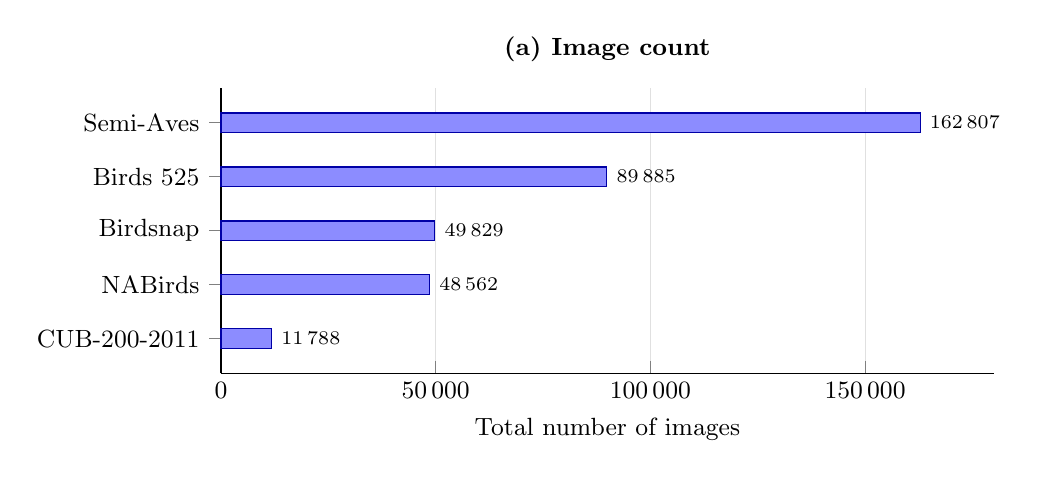
\begin{tikzpicture}
        \begin{axis}[
            width=0.94\textwidth,
            height=5.2cm,
            xbar,
            bar width=7pt,
            xmin=0,
            xmax=180000,
            xtick={0,50000,100000,150000},
            scaled x ticks=false,
            xticklabel style={
                /pgf/number format/fixed,
                /pgf/number format/1000 sep={\,}
            },
            xlabel={Total number of images},
            ytick={1,2,3,4,5},
            yticklabels={
                CUB-200-2011,
                NABirds,
                Birdsnap,
                Birds 525,
                Semi-Aves
            },
            yticklabel style={font=\small},
            tick label style={font=\small},
            label style={font=\small},
            axis x line*=bottom,
            axis y line*=left,
            xmajorgrids=true,
            grid style={draw=black!12},
            enlarge y limits=0.16,
            nodes near coords={
                \pgfmathprintnumber[
                    fixed,
                    precision=0,
                    1000 sep={\,}
                ]{\pgfplotspointmeta}
            },
            nodes near coords align={horizontal},
            every node near coord/.append style={
                font=\scriptsize,
                anchor=west
            },
            point meta=x,
            clip=false,
            title={(a) Image count},
            title style={font=\small\bfseries}
        ]
            \addplot[
                draw=blue!65!black,
                fill=blue!45
            ] coordinates {
                (11788,1)
                (48562,2)
                (49829,3)
                (89885,4)
                (162807,5)
            };
        \end{axis}
    \end{tikzpicture}

    \vspace{0.5em}

    % Class-count chart
    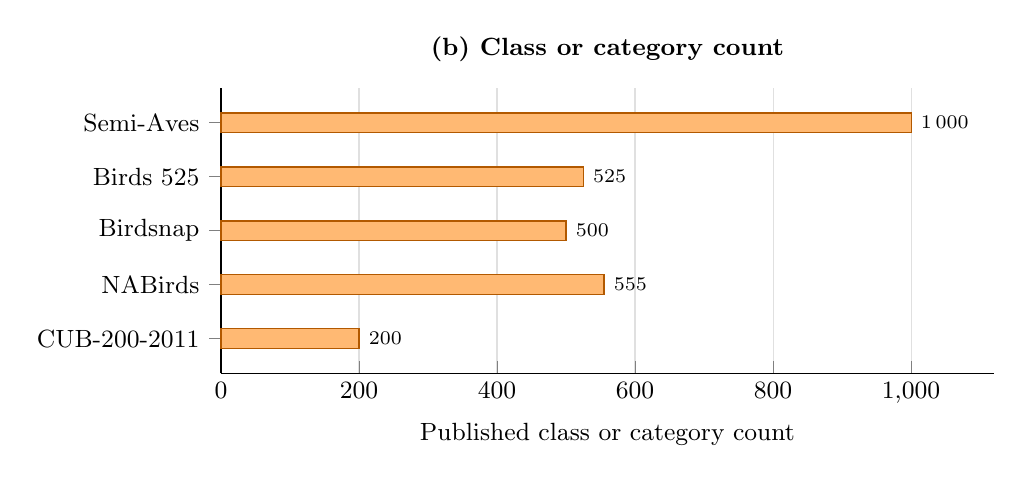
\begin{tikzpicture}
        \begin{axis}[
            width=0.94\textwidth,
            height=5.2cm,
            xbar,
            bar width=7pt,
            xmin=0,
            xmax=1120,
            xtick={0,200,400,600,800,1000},
            scaled x ticks=false,
            xlabel={Published class or category count},
            ytick={1,2,3,4,5},
            yticklabels={
                CUB-200-2011,
                NABirds,
                Birdsnap,
                Birds 525,
                Semi-Aves
            },
            yticklabel style={font=\small},
            tick label style={font=\small},
            label style={font=\small},
            axis x line*=bottom,
            axis y line*=left,
            xmajorgrids=true,
            grid style={draw=black!12},
            enlarge y limits=0.16,
            nodes near coords={
                \pgfmathprintnumber[
                    fixed,
                    precision=0,
                    1000 sep={\,}
                ]{\pgfplotspointmeta}
            },
            nodes near coords align={horizontal},
            every node near coord/.append style={
                font=\scriptsize,
                anchor=west
            },
            point meta=x,
            clip=false,
            title={(b) Class or category count},
            title style={font=\small\bfseries}
        ]
            \addplot[
                draw=orange!70!black,
                fill=orange!55
            ] coordinates {
                (200,1)
                (555,2)
                (500,3)
                (525,4)
                (1000,5)
            };
        \end{axis}
    \end{tikzpicture}

    \caption[
        Comparison of the scale of selected bird-image datasets
    ]{
        Scale of selected bird-image datasets by total image count
        and published class or category count. Adapted from dataset
        statistics reported by Wah et al. \cite{WahEtAl2011},
        Van Horn et al. \cite{VanHornEtAl2015},
        Berg et al. \cite{BergEtAl2014},
        Gpiosenka \cite{Birds525Dataset}, and
        Su and Maji \cite{SuMaji2021}.
    }
    \label{fig:bird-dataset-scale}

    \vspace{0.4em}
\end{figure}

A smaller class set introduces the challenge of handling unidentified birds and other off-target detections. Two scenarios must be considered: low-confidence predictions and classes unknown to the model. Low-confidence predictions can be handled using selective classification, or a "reject option", in which predictions below a confidence threshold are rejected \cite{GeifmanElYaniv2017}. Unknown classes arise because the model operates in an open-set environment, where it may encounter classes absent from its training data \cite{ScheirerEtAl2013}. A similar rejection mechanism should therefore be used to prevent unreliable classification of unknown visitors.


\subsection{Embedded and autonomous usage}

%\begin{itemize}
%    \item \sout{Advantages of edge processing.}
%    \item \sout{General computational and energy constraints.}
%    \item \sout{Solar-powered wildlife-monitoring systems.}
%\end{itemize}

Given that this project aims to rely on solar power for continuous remote operation, literature concerning its embedded and autonomous functionality must also be reviewed.
\par\vspace{6pt}
While most existing smart feeders discussed previously rely on external servers or cloud services for data storage and processing, this project will instead perform these functions on-device using edge processing. Besides removing dependence on remote processing, edge processing enables immediate decisions on whether footage should be recorded, reducing storage of irrelevant data \cite{DarrasEtAl2024}.
\par\vspace{6pt}
This project requires an inference model capable of identifying bird visits quickly enough to determine whether recording should occur. Microcontrollers offer low-power operation and are well suited to simple sensing and processing, but their limited architecture restricts demanding tasks such as inference and image classification. Consequently, these tasks generally take considerably longer than on a microcomputer, limiting the suitability of microcontrollers for neural-network applications \cite{BallerEtAl2021}.
\par\vspace{6pt}
Microcomputers provide greater processing capability but require significantly more power while operating. Trigger-based recording can reduce storage requirements, but will only similarly reduce power consumption if components, or the system as a whole, can enter and exit an idle state when inactive \cite{BalleEtAl2025}. The principal differences between conventional microcontrollers and Raspberry Pi--class single-board computers are summarised in Table~\ref{tab:microcontroller-sbc-comparison}.

\par\vspace{6pt}

\begin{table}[htbp]
    \centering
    \caption{Comparison of conventional microcontrollers and Raspberry Pi--class single-board computers.}
    \label{tab:microcontroller-sbc-comparison}

    \footnotesize
    \setlength{\tabcolsep}{4pt}
    \renewcommand{\arraystretch}{1.2}

    \begin{tabularx}{\textwidth}{
        >{\raggedright\arraybackslash}p{0.13\textwidth}
        >{\raggedright\arraybackslash}X
        >{\raggedright\arraybackslash}X
        >{\raggedright\arraybackslash}p{0.22\textwidth}
    }
        \toprule
        \textbf{Criterion}
        & \textbf{Microcontroller}
        & \textbf{Raspberry Pi--class SBC}
        & \textbf{Project relevance} \\
        \midrule

        Power
        & Very low consumption with effective sleep modes.
        & Typically consumes several watts when active.
        & Microcontrollers offer better low-power operation. \\

        \addlinespace

        Start-up
        & Begins operating almost immediately.
        & Requires several seconds to boot.
        & Frequent SBC power cycling may delay capture. \\

        \addlinespace

        Memory
        & Usually kilobytes to a few megabytes.
        & Commonly provides several gigabytes.
        & Video processing requires SBC-level memory. \\

        \addlinespace

        Camera and video
        & Limited resolution and video-handling capability.
        & Supports high-resolution cameras and sustained video capture.
        & Short-video recording favours the SBC. \\

        \addlinespace

        Machine learning
        & Restricted mainly to compact TinyML models.
        & Supports larger models and inference accelerators.
        & Species classification favours the SBC. \\

        \addlinespace

        Software
        & Runs embedded firmware or a real-time operating system.
        & Runs Linux with established camera and ML libraries.
        & The SBC simplifies system integration. \\

        \addlinespace

        Data and web access
        & Storage, databases and web services are constrained.
        & Supports local storage, databases and web servers.
        & Required for visit logging and the web interface. \\

        \addlinespace

        Reliability
        & Simple software stack and rapid recovery.
        & Requires storage, thermal and shutdown management.
        & SBC reliability must be addressed in the design. \\

        \midrule

        Recommended role
        & Optional trigger or power-management controller.
        & \textbf{Primary system processor.}
        & Add a microcontroller only if testing demonstrates a need. \\

        \bottomrule
    \end{tabularx}

    \vspace{0.4em}
\end{table}

For a system to operate continuously using only solar power, the usable solar energy generated must meet or exceed the system's energy demand and associated losses:

$$
E_{\text{solar, usable}} \geq E_{\text{system}} + E_{\text{losses}}
$$

\par\vspace{6pt}
Although most smart feeders reviewed previously rely on external power, commercial products such as the Birdfy and academic studies demonstrate that solar-powered operation is feasible \cite{BirdfyHumFeeder,PouRossellEtAl2025}.
\par\vspace{6pt}
Having investigated the key technologies supporting the proposed system, a clearer basis for the design phase has been established. The advantages and limitations of each technology have been considered to identify the options most suitable for this project.

\section{Conclusion}

With the relevant literature investigated, several conclusions can be drawn to support the motivation for this research and inform the design and methods of the proposed system.
\par\vspace{6pt}
Analysis of existing smart bird feeders provides insight into existing solutions and opportunities for improvement. Many systems use neural-network classification to automate non-invasive species identification. However, several rely on external processing, cloud services or network connectivity, limiting their suitability for remote deployment. Similarly, fully autonomous solar operation is not consistently demonstrated. These limitations support the use of local processing, storage and power generation in this project.
\par\vspace{6pt}
The review also identified relatively little research on smart nectar feeders, with most literature focused on seed feeders despite several commercial hummingbird feeders. Focusing on nectar-feeding birds introduces additional design considerations, including feeder colour, nectar replacement and protecting electronic components from nectar spillage and environmental exposure.
\par\vspace{6pt}
In conclusion, the literature reviewed proves the feasibility of the required technology for this project, but these proofs are hardly realised as a combined and complete smart nectar feeder for sunbirds. The findings from the literature support the use of triggered video capture, a locally relevant classification model, edge computing and local storage, together with autonomous solar power.
The basis for the system requirements and design decisions developed in the following chapters will be constructed using these findings.